%%%%% --------------------------------------------------------------------------------
%%
%%                               Beamer Theme
%%
%%%%% --------------------------------------------------------------------------------
%% Copyright (C) Huangrui Mo <huangrui.mo@gmail.com>
%% This is free software: you can redistribute it and/or modify it
%% under the terms of the GNU General Public License as published by
%% the Free Software Foundation, either version 3 of the License, or
%% (at your option) any later version.
%%%%% --------------------------------------------------------------------------------
%%
%%%%************************* Beamer Class Declaration *******************************
%%
\documentclass[compress,table,xcolor={usenames,dvipsnames}]{beamer}
%% Multiple Options:
%% [<t|c|b>] % vertical alignment for silde content, vertically centerred is default
%% [<slidestop|slidescentered>] % set frame titles position
%% [compress] % reduce the navigate bars
%% [<red|blue|brown|blackandwhite>] % set navigate bar color
%% [<11pt|12pt|17pt>] % set font size, 11pt is default
%% [table] % support tables
%% [aspectratio=1610] % set aspect ratio to 16:10, and frame size to 160mm by 100mm
%% [aspectratio=MN] % set aspect ratio to M:N, and frame size to 10*M mm by 10*N mm
%% [xcolor={usenames,dvipsnames}] % issue options to xcolor via a beamer-option.
%%%%% --------------------------------------------------------------------------------
%%
%%%%************************* Command Define and Settings ****************************
\usepackage[tikz,table]{commons}% common settings
%% Multiple Options:
%% [CJK] % support Chinese environment
%% [tikz] % support tikz for graphics
%% [table] % enable some table packages
%% [list] % verbatim environments
%% [handout] % enable handout output
\usepackage{custom}% user defined commands and settings
%% Multiple Options:
%% [showonlynote] % show note pages only
%% [showsecnote] % show note pages on second screen
%%%%% --------------------------------------------------------------------------------
%%
%%%%**************************** Themes Setting **************************************
%%
%%% >>> Global Themes
%%
\usetheme{CambridgeUS}
%% Options:
%% [<Szeged|Singapore|Madrid|CambridgeUS|...>]
%% It is the complete theme in the sense that they control just about every aspect
%% of a slide's appearance. Think of it as major theme.
%% The Theme Matrix (https://www.hartwork.org/beamer-theme-matrix/) contains the
%% various theme and color combinations included with beamer.
%%
%%% >>> Outer Themes
%%
%\useoutertheme{}
%% Options:
%% [<default|infolines|miniframes|smoothbars|sidebar|split|shadow|tree|smoothtree>]
%% An outer theme dictates (roughly) the overall layout of frames. It specifies where
%% any navigational elements should go (like a mini table of contents or navigational
%% mini frames) and what they should look like. Typically, an outer theme specifies
%% how the following elements are rendered:
%% - The headline and footline.
%% - The sidebars.
%% - The logo.
%% - The frame title.
%% The Beamer User Guide explains each theme with examples.
%%
%% *** Miniframes
\useoutertheme[%
%   footline=empty, % suppressed the footline (default).
%   footline=authorinstitute, % shows the author's name and the institute in the footline.
%   footline=authortitle, % shows the author's name and the title in the footline.
%   footline=institutetitle, % shows the institute and the title in the footline.
%   footline=authorinstitutetitle, % shows all three in the footline.
    subsection=false, % shows or suppresses line showing the subsection in the headline.
    ]{miniframes}
%%
%% *** Sidebar
%\useoutertheme[%
%   left, % sidebar links
%   right, % sidebar rechts
%   hideallsubsections, % suppresses all subsections
%   hideothersubsections, % suppresses all subsections except the current one
%   ]{sidebar}
%%
%%% >>> Inner Themes
%%
\useinnertheme{circles}
%% Options:
%% [<default|circles|rectangles|rounded|inmargin>]
%% An inner theme installs templates that dictate how the following elements are typeset:
%% - Title and part pages.
%% - Itemize environments.
%% - Enumerate environments.
%% - Description environments.
%% - Block environments.
%% - Theorem and proof environments.
%% - Figures and tables.
%% - Footnotes.
%% - Bibliography entries.
%%
%%% >>> Color Themes
%%
\usecolortheme{seagull}
%% Options:
%% [<seahorse|seagull|beaver|rose|dove|lily|orchid|crane|beetle|fly>]
%% Control the colors of title, frame title, itemization bullets,
%% and many other elements of a slide show.
%% More detailed configure:\setbeamercolor{beamer_element}{color} for
%% of Beamer elements, e.g.color setup
%\setbeamercolor{title}{fg=red!80!black,bg=red!20!white}
%\setbeamercolor{frametitle}{fg=blue,bg=yellow}
%%%%% --------------------------------------------------------------------------------
%%
%%%%******************************* Template Configure *******************************
%%
%%% >>> Set Templates
%%
%% As a user of the beamer class you typically do not 'use' or 'invoke'
%% templates yourself, directly. For example, the frame title template
%% is automatically invoked by beamer somewhere deep inside the frame
%% typesetting process. The same is true of most other templates.
%% However, if, for whatever reason, you wish to invoke a template
%% yourself, you can use the following command.
%%\setbeamertemplate{some beamer element}{your definition for this template}
%%
%% *** The Headline and Footline
%\setbeamertemplate{headline}[infolines theme]
%\setbeamertemplate{footline}[page number]
%% Options: {},[default],[infolines theme],[miniframes theme],[frame number],
%%          [page number],[text line]{ text },...
%% Example for redefine the footline:
%%
%%% First define some "beamer color" entries:
%\setbeamercolor{myentry1}{fg=black,bg=red!20}
%\setbeamercolor{myentry2}{fg=black,bg=red!30}
%\setbeamercolor{myentry3}{fg=black,bg=red!40}
%%% Syntax for \begin{beamercolorbox}[options]{beamer color} ... \end{beamercolorbox}.
%%% footline:
%\setbeamertemplate{footline}{
%  \leavevmode%
%  \hbox{%
%  \begin{beamercolorbox}[wd=.333333\paperwidth,ht=2.25ex,dp=1ex,center]{myentry1}%
%%    \usebeamerfont{author in head/foot}\insertshortauthor
%  \end{beamercolorbox}%
%  \begin{beamercolorbox}[wd=.333333\paperwidth,ht=2.25ex,dp=1ex,center]{myentry2}%
%%    \usebeamerfont{title in head/foot}\insertshorttitle
%  \end{beamercolorbox}%
%  \begin{beamercolorbox}[wd=.333333\paperwidth,ht=2.25ex,dp=1ex,right]{myentry3}%
%%    \usebeamerfont{date in head/foot}\insertshortdate{}\hspace*{2em}
%    \insertframenumber{} / \inserttotalframenumber\hspace*{2ex}
%  \end{beamercolorbox}}%
%  \vskip0pt%
%}
%%% headline:
%\setbeamertemplate{headline}{
%  \leavevmode%
%  \hbox{%
%  \begin{beamercolorbox}[wd=.5\paperwidth,ht=2.65ex,dp=1.5ex,right]{myentry1}%
%    \usebeamerfont{section in head/foot}\insertsectionhead\hspace*{2ex}
%  \end{beamercolorbox}%
%  \begin{beamercolorbox}[wd=.5\paperwidth,ht=2.65ex,dp=1.5ex,left]{myentry3}%
%    \usebeamerfont{subsection in head/foot}\hspace*{2ex}\insertsubsectionhead
%  \end{beamercolorbox}}%
%  \vskip0pt%
%}
%% Change the footer/footline of a single frame in Beamer: use {} to confine effect domain.
%% The \leavevmode ensures that the vertical mode is ended and horizontal mode is entered. 
%% In vertical mode, TeX stacks horizontal boxes vertically, whereas in horizontal mode, 
%% they are taken as part of the text line. Use \leavevmode for all macros which could be 
%% used at the begin of the paragraph and add horizontal boxes by themselves.
%%
%% *** The Outline Setting
%\AtBeginSection[] % [<AtBeginSection|AtBeginSubsection>]
%{
%  \begin{frame}<beamer>[plain]
%    \frametitle{Outline}
%    {
%     \tableofcontents[sectionstyle=show/shaded,subsectionstyle=show/show/shaded]
%    }
%  \end{frame}
%}
%% - sectionstyle=<style for current section>/<style for other sections>
%% - subsectionstyle=<style for current subsection>/<style for other
%%   subsections in current section>/<style for subsections in other sections>
%% - Allowed <styles> are show, shaded, and hide.
%% Other Options:
%% - currentsection, equal to: sectionstyle=show/shaded,subsectionstyle=show/show/shaded
%% - currentsubsection, equal to: subsectionstyle=show/shaded.
%% - firstsection=<section number> specifies which section should be numbered as section “1.”
%%   This is useful if you have a first section (like an overview section) that should not
%%   receive a number.
%% - hideallsubsections, equal to: subsectionstyle=hide.
%% - pausesections, causes a \pause command to be issued before each section.
%%   This is useful if you wish to show the table of contents in an incremental way.
%%
%% *** The Navigation Symbols
\setbeamertemplate{navigation symbols}{} % suppresses all navigation symbols.
%\setbeamertemplate{navigation symbols}[only frame symbol] % only for navigating frames.
%%
%% *** The Frame Title
%\setbeamertemplate{frametitle}[default][left] % left, center, right
%%
%% *** The Background
%\setbeamertemplate{background canvas}[default]
%\setbeamertemplate{background canvas}[vertical shading][bottom=red!20,top=yellow!30]
%\setbeamertemplate{background canvas}{\includegraphics[width=\paperwidth,height=\paperheight]{alps.jpg}}
%% The aspect ratio of a Beamer slide is 4:3 therefore it's best
%% if your background image has the same aspect ratio. Otherwise
%% your image will be distorted when it's stretched to cover the
%% slide from edge to edge.
%% To limit the background setting to a single slide, enclose the
% \setbeamertemplate{background canvas}{...} command in braces,
%% as in:
%%
%{ % brace to limit the scope of \setbeamertemplate
%\setbeamertemplate{navigation symbols}{} % optionally hide navigation buttons
%\setbeamertemplate{background canvas}{\includegraphics
%	[width=\paperwidth,height=\paperheight]{alps.jpg}}
%\begin{frame}[plain]
%...
%\end{frame}
%} % closing brace
%%
%% *** Margin Sizes
%\setbeamersize{text margin left=2em,text margin right=2em}
%%
%% *** Itemizations, Enumerations, and Descriptions
%\setbeamertemplate{itemize items}[triangle]
%% Options: [<circle|triangle|square|ball>].
%\setbeamertemplate{enumerate items}[default]
%% Options:
%% [default] % numbered
%% [sections numbered] % section numbered, subsections are not numbered.
%% [subsections numbered] % subsections are numbered, but not the sections.
%% [circle] % numbered circles before section, not subsection.
%% [square] % numbered squares before section. unnumbered squares before subsections.
%% [ball] % similar to square, but use balls.
%% [ball unnumbered] % similar to ball, except that no numbering is used.
%%
%% *** Block Environments
%\setbeamertemplate{blocks}[rounded][shadow=true]
%% Types:
%% "theorem", "corollary", "definition" in structure color frame.
%% "examples" in green color frame.
%% "block" in structure color frame with your own title.
%% "alertblock" in alert color frame with your own title.
%%
%% *** Theorem Environments
%\setbeamertemplate{theorems}[normal font]
%% Options: [<default|normal font|numbered|ams style>].
%%
%% *** Figures and Tables
%\setbeamertemplate{caption}[default]
%% Options:
%% [default] % typesets the caption name (a word like 'Figure' or 'Abbildung' or 'Table')
%% [numbered] % adds the figure or table number to the caption.
%% [caption name own line].
%%
%% *** Adding Sections and Subsections
%\setbeamertemplate{sections/subsections in toc}[square]
%% Options: [<default|sections numbered|subsections numbered>]
%%          [<circle|square|ball|ball unnumbered>]
%%
%% *** Bibliography
\setbeamertemplate{bibliography item}{} % remove the icon
%%
%%% >>> Set Fonts
%%
%% Rules:
%\setbeamerfont{some beamer element}{size=\large}
%% Add a star to the command to first “reset” the font.
%% Options:
%% parent=structure,size=\large,series=\bfseries,shape=\itshape,family=\sffamily.
%% Explains: there are three familis of font
%% family: \rmfamily(serif) or \sffamily(sans serif), or \ttfamily(monospace).
%% Each family has its own font characteristics, i.e., font properties.
%% shapes: \itshape, \slshape, \scshape, or \upshape.
%% series(light, bold,...): \bfseries, \mdseries.
%%
%% *** Structure Font
%\setbeamerfont{structure}{}
%\setbeamerfont{tiny structure}{size=\tiny}
%%
%% *** Normal Font
%\setbeamerfont{normal text}{parent=structure,size=\small} % ignored currently
%\setbeamerfont{alerted text}{}
%\setbeamerfont{example text}{}
%%
%% *** Projected Text Font
%\setbeamerfont{projected text}{parent={tiny structure}}
%%
%% *** Titlepage Font
%\setbeamerfont{title}{parent=structure, size=\large} % shape=\itshape,family=\rmfamily
%\setbeamerfont{title in head/foot}{parent=title, size=\tiny}
%\setbeamerfont{subtitle}{parent=title, size=\normalsize}
%\setbeamerfont{author}{parent=title, size=\normalsize}
%\setbeamerfont{author in head/foot}{parent=title, size=\tiny}
%\setbeamerfont{institute}{parent=structure, size=\scriptsize, series=\mdseries}
%\setbeamerfont{institute in head/foot}{parent=title, size=\tiny}
%\setbeamerfont{date}{parent=institute}
%\setbeamerfont{date in head/foot}{parent=title, size=\tiny}
%%
%% *** Frame Title Font
\setbeamerfont{frametitle}{parent=structure,size=\large}
%\setbeamerfont{framesubtitle}{parent=frametitle,size=\footnotesize}
%%
%% *** Part Fonts
%\setbeamerfont{part name}{size=\Large}
%\setbeamerfont{part title}{parent=title}
%%
%% *** Headline and Footline Font
%\setbeamerfont{headline}{parent={tiny structure}}
%\setbeamerfont{footline}{parent={tiny structure}}
%%
%% *** Caption Font
%\setbeamerfont{caption}{size=\small}
%\setbeamerfont{caption name}{size=\small}
%%
%% *** Button Font
%\setbeamerfont{button}{size=\tiny}
%%
%%% >>> Transparent Effect
%%
%\setbeamercovered{invisible}
%% Options:
%% [invisible] % is the default and causes covered text to disappear.
%% [transparent] % creates shaded instead of hidden overlays.
%% [dynamic] % makes all covered text quite transparent, but in a dynamic way.
%% [highly dynamic] % has the same effect as dynamic, but the effect is stronger.
%\beamerdefaultoverlayspecification{<+->} % uncover everything in a step-wise fashion
%%%%% --------------------------------------------------------------------------------
%%
%%%%******************************** Content *****************************************
%%
\begin{document}
%%
%%% >>> Front Page Info
%%
%%%%% --------------------------------------------------------------------------------
%%
%%%%*****************************Title Page Info*************************************
%%
\title[]%[Beamer Guide] % optional, use only with long paper titles
{How to Make Presentation by Beamer}
%%
\subtitle
{ - An Introduction}
%%
\author[] % optional, use only with lots of authors
{Huangrui Mo}
%% Example:
%\author[Author, Another]
%{F.~Author\inst{1} \and S.~Another\inst{2}}
% Give the names in the same order as the appear in the paper.
% Use the \inst{?} command only if the authors have different
% affiliation.
%%
\institute[]% % optional, but mostly needed
{
  University of Waterloo
}
%% Example:
%\institute[Universities of Somewhere and Elsewhere]
%{
%  \inst{1}%
%  Department of Computer Science\\
%  University of Somewhere
%  \and
%  \inst{2}%
%  Department of Theoretical Philosophy\\
%  University of Elsewhere
%}
%% Use the \inst command only if there are several affiliations.
%% Keep it simple, no one is interested in your street address.
%%
\date[]
{\today}
%% Example:
%\date[CFP 2003] % optional, should be abbreviation of conference name
%{Conference on Fabulous Presentations, 2003}
%% Either use conference name or its abbreviation.
%% Not really informative to the audience, more for people (including
%% yourself) who are reading the slides online.
%% or simply use: \date{\today}
%%
%% This is only inserted into the PDF information catalog. Can be left out.
\subject{Beamer}
%%
%\logo{
\includegraphics[height=0.10\textwidth]{Logo}}
%
%%
%%% >>> Main Content
%%
%%%%% ++++++++++++++++++++++++++++++++++++++++++++++++++++++++++++++++++++++++
%%
%%% >>> Create Title Page
%%
%%%%% ++++++++++++++++++++++++++++++++++++++++++++++++++++++++++++++++++++++++
%% Create the title page, \frame[plain]{\titlepage} for a titlepage filling the whole frame.
{ % these braces make the change local to the single frame.
    \setbeamertemplate{headline}{%
        \begin{beamercolorbox}[wd=\paperwidth,ht=2.5ex,dp=1.5ex,right]{section in head/foot}%
        \end{beamercolorbox}%
    }
    \setbeamertemplate{footline}{%
        \leavevmode%
        \hbox{%
            \begin{beamercolorbox}[wd=.333333\paperwidth,ht=2.25ex,dp=1ex,center]{author in head/foot}%
            \end{beamercolorbox}%
            \begin{beamercolorbox}[wd=.333333\paperwidth,ht=2.25ex,dp=1ex,center]{title in head/foot}%
            \end{beamercolorbox}%
            \begin{beamercolorbox}[wd=.333333\paperwidth,ht=2.25ex,dp=1ex,right]{date in head/foot}%
            \end{beamercolorbox}}%
        \vskip0pt%
    }
    \begin{frame}%[plain]
        \titlepage%
        \note{
            \begin{itemize}
                \item Good afternoon everyone.
                \item In the next 15 minutes, I would like to present you my research on "..."
            \end{itemize}
        }
    \end{frame}%
    %% Modified the framenumber counter so that the frames including the footline start from one.
    \addtocounter{framenumber}{-1}%
}
%%%%% ++++++++++++++++++++++++++++++++++++++++++++++++++++++++++++++++++++++++
%%
%%% >>> Outline page
%%
%%%%% ++++++++++++++++++++++++++++++++++++++++++++++++++++++++++++++++++++++++
%\section[Outline]{}%
%\begin{frame}%[plain]%
%    \frametitle{Outline}%
%    \tableofcontents% you might wish to add the option [pausesections]
%    \note{
%        \begin{itemize}
%            \item Introduction: introduce the research problem and objectives.
%            \item Methodology: describe the methodology for addressing the research problem.
%            \item Results: demonstrate the research methodology.
%            \item Conclusions: summarize the presentation.
%        \end{itemize}
%    }
%\end{frame}%
%%%%% ++++++++++++++++++++++++++++++++++++++++++++++++++++++++++++++++++++++++
%%
%%% >>> Contents
%%
%%%%% ++++++++++++++++++++++++++++++++++++++++++++++++++++++++++++++++++++++++
%\centering % automatic horizontal centering of frame content
%%%%% ++++++++++++++++++++++++++++++++++++++++++++++++++++++++++++++++++++++++
\section{Why Beamer}
%%%%% ++++++++++++++++++++++++++++++++++++++++++++++++++++++++++++++++++++++++++++++
\begin{frame}[fragile]
\frametitle{Why Beamer}

  Pros:

  \begin{itemize}
    \item Both \textcolor{magenta}{dvips/ps2pdf} and \textcolor{magenta}{pdflatex} supports
    \item Rich \textcolor{magenta}{overlay} and \textcolor{magenta}{transition} effects
    \item Navigational bars and symbols
    \item Outputs: screen, transparency, handouts, and notes
    \item Emulation of other PDF presetation tools such as Prosper
    \item Easy to type math
    \item \path{WYSIWYM} (What You See Is What You Mean)
  \end{itemize}

  Cons:

  \begin{itemize}
    \item Not \path{WYSIWYG} (What You See Is What You Get)
    \item Steep learning curve
    \item Difficult to design a template
  \end{itemize}

\end{frame}
%%%%% ++++++++++++++++++++++++++++++++++++++++++++++++++++++++++++++++++++++++++++++
\section{Creating a Slideshow}
%%%%% ++++++++++++++++++++++++++++++++++++++++++++++++++++++++++++++++++++++++++++++
\subsection{Examples}
%%%%% ++++++++++++++++++++++++++++++++++++++++++++++++++++++++++++++++++++++++++++++
\begin{frame}[fragile]
\frametitle{My First Slide}
  \begin{footnotesize}
    \begin{verbatim}
\documentclass{beamer}
\begin{document}
  \begin{frame}
    Hello World!
  \end{frame}
\end{document}
    \end{verbatim}
  \end{footnotesize}
\end{frame}
%%%%% ++++++++++++++++++++++++++++++++++++++++++++++++++++++++++++++++++++++++++++++
\subsection{Titles}
%%%%% ++++++++++++++++++++++++++++++++++++++++++++++++++++++++++++++++++++++++++++++
\begin{frame}[fragile]
\frametitle{Frame Titles}
\framesubtitle{...and Subtitles}

  Two ways to create titles and subtitles for a frame:

  \begin{itemize}
    \item \verb|\begin{frame}{|\emph{Frame Title}\verb|}{|\emph{Frame Subtitle}\verb|}|
    \item \verb|\frametitle{|\emph{Frame Title}\verb|}\framesubtitle{|\emph{Frame Subtitle}\verb|}|
  \end{itemize}

\end{frame}
%%%%% ++++++++++++++++++++++++++++++++++++++++++++++++++++++++++++++++++++++++++++++
\subsection{Sections}
%%%%% ++++++++++++++++++++++++++++++++++++++++++++++++++++++++++++++++++++++++++++++
\begin{frame}[fragile]
\frametitle{Sectioning}

  Notice the sections and subsections at the top of each slide.

  \begin{footnotesize}
    \begin{itemize}
      \item \verb|\section[|\emph{Short Section Name}\verb|]{|\emph{Long Section Name}\verb|}|
      \item \verb|\subsection[|\emph{Short Subsection Name}\verb|]{|\emph{Long Subsection Name}\verb|}|
    \end{itemize}
  \end{footnotesize}

  \vskip .2in

  \uncover<2->{``Short names'' go into slide headers;\\
  ``Long names'' go into outlines.}

  \vskip .2in

  \uncover<3->{All sections and subsections automatically added to slideshow outline!}

\end{frame}
%%%% ++++++++++++++++++++++++++++++++++++++++++++++++++++++++++++++++++++++++++++++
\begin{frame}[fragile]
\frametitle{Loooooong Slides}

  \textsc{Beamer} does not automatically put what doesn't fit from one slide onto another slide.

  \begin{itemize}
    \item You must keep track of slide lengths yourself; or
    \item you can use the frame option \verb|\begin{frame}[allowframebreaks]|
  \end{itemize}

  This automatically breaks up the long slide and puts the extra content onto new slides.

  \bigskip

  \uncover<2->{\alert<2->{\path{+}} You don't have to worry about the length of your slides.}

  \uncover<3->{\alert<3->{\path{+}} Slide title is continued on each subsequent slide.}

  \uncover<4->{\alert<4->{\path{-}} Most overlay options are not usable.}

\end{frame}
%%%%% ++++++++++++++++++++++++++++++++++++++++++++++++++++++++++++++++++++++++++++++
\subsection{Use Verbatim}
%%%%% ++++++++++++++++++++++++++++++++++++++++++++++++++++++++++++++++++++++++++++++
\begin{frame}[fragile]
\frametitle{Verbatim}

  \begin{tiny}
    \begin{semiverbatim}
      \uncover<1->{int main (void)} \uncover<1->{\{}
      \uncover<1->{std::vector<bool> is_prime (100, true);}
      \uncover<1->{ for (int i = 2; i < 100; i++)}
      \uncover<2->{{ if (is_prime[i])}}
      \uncover<2->{\{} \uncover<3->{ std::cout << i << " ";}
      \uncover<3->{ for (int j = i; j < 100;}
      \uncover<3->{ is_prime [j] = false, j+=i);}
      \uncover<2->{ \}} \uncover<1->{ return 0;}
      \uncover<1->{\}}
    \end{semiverbatim}
  \end{tiny}

  \pause\pause\pause

  \begin{block}{Using Verbatim}
    To use any sort of verbatim text, you must declare the frame as \textsl{fragile}:\\ \verb|\begin{frame}[fragile]|\\
    Use \verb|\path{content}|, \path{\verb |content|} or \verb|verbatim| environment.
  \end{block}

\end{frame}
%%%%% ++++++++++++++++++++++++++++++++++++++++++++++++++++++++++++++++++++++++++++++
\subsection{Use Enumerate}
%%%%% ++++++++++++++++++++++++++++++++++++++++++++++++++++++++++++++++++++++++++++++
\begin{frame}[fragile]
\frametitle{Enumerate}

  \begin{enumerate}[A]
    \item This is the first item.
    \item This is the second item.
    \item Yes, this is the third one!
  \end{enumerate}

  \vfill

  \begin{footnotesize}
    \begin{verbatim}
\begin{enumerate}[minitemplate]
  \item ...
\end{enumerate}
where minitemplate can be empty or 'A','a', 'i', 'I', '(A)', ...
    \end{verbatim}
  \end{footnotesize}

\end{frame}
%%%%% ++++++++++++++++++++++++++++++++++++++++++++++++++++++++++++++++++++++++++++++
\subsection{Framed Text}
%%%%% ++++++++++++++++++++++++++++++++++++++++++++++++++++++++++++++++++++++++++++++
\begin{frame}[fragile]
\frametitle{Framed Text}

  \begin{theorem}
    You can read this.
  \end{theorem}

  \begin{alertblock}{Warning}
    You are warned!
  \end{alertblock}

  \vfill

  Beamer supports predefined framed texts:

  \begin{footnotesize}
    \begin{verbatim}
theorem, corollary, definition in structure color frame
examples in green color frame
block in structure color frame with your own title
alertblock in alert color frame with your own title
    \end{verbatim}
  \end{footnotesize}

\end{frame}
%%%%% ++++++++++++++++++++++++++++++++++++++++++++++++++++++++++++++++++++++++++++++
\begin{frame}[fragile]
\frametitle{User-defined Framed Text}

{
  \setbeamercolor{uppercol}{fg=white,bg=green!80}%
  \setbeamercolor{lowercol}{fg=black,bg=green!10}%
  \begin{beamerboxesrounded}[upper=uppercol,lower=lowercol,shadow=true]{Theorem}
    $A = B$.
  \end{beamerboxesrounded}
}

  \vfill

  Source code:

  \begin{footnotesize}
    \begin{verbatim}
{
\setbeamercolor{uppercol}{fg=white,bg=green!80}%
\setbeamercolor{lowercol}{fg=black,bg=green!10}%
\begin{beamerboxesrounded}%
[upper=uppercol,lower=lowercol,shadow=true]{Theorem}
  $A = B$.
\end{beamerboxesrounded}
}
    \end{verbatim}
  \end{footnotesize}

\end{frame}
%%%%% ++++++++++++++++++++++++++++++++++++++++++++++++++++++++++++++++++++++++++++++
\section{Graphics}
%%%%% ++++++++++++++++++++++++++++++++++++++++++++++++++++++++++++++++++++++++++++++
\begin{frame}[fragile]
\frametitle{\path{\includegraphics{}}}

  \begin{columns}
    \begin{column}{.5\textwidth}
      \begin{tiny}
        \begin{verbatim}
\begin{columns}
\begin{column}{.5\textwidth}
  \centering
  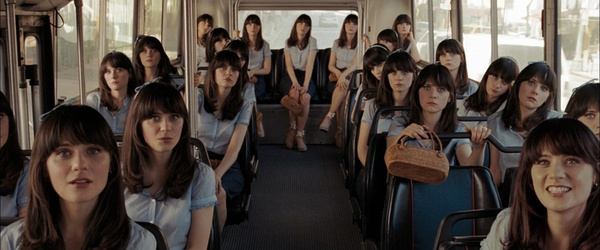
\includegraphics[width=\textwidth]{Zooey1}
\end{column}
\begin{column}{.5\textwidth}
  \centering
  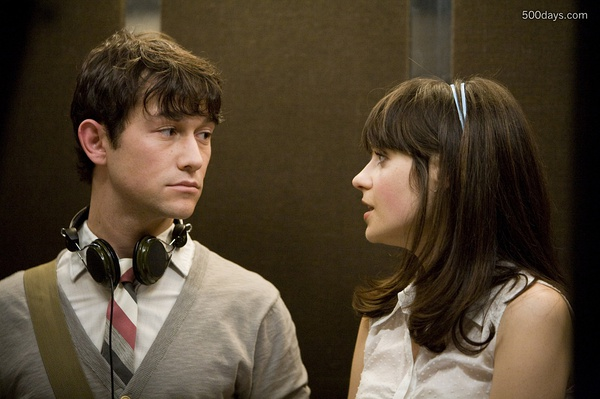
\includegraphics[width=\textwidth]{Zooey2}
\end{column}
\end{columns}
        \end{verbatim}
      \end{tiny}
    \end{column}

    \begin{column}{.5\textwidth}
      \begin{columns}
        \begin{column}{.5\textwidth}
          \centering
          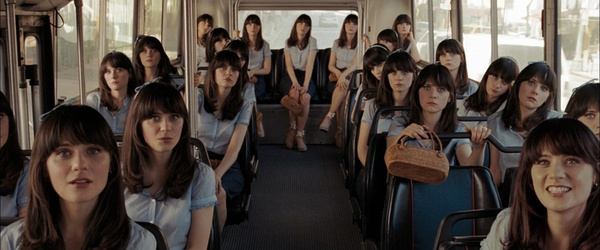
\includegraphics[width=\textwidth]{Zooey1}
        \end{column}
        \begin{column}{.5\textwidth}
          \centering
          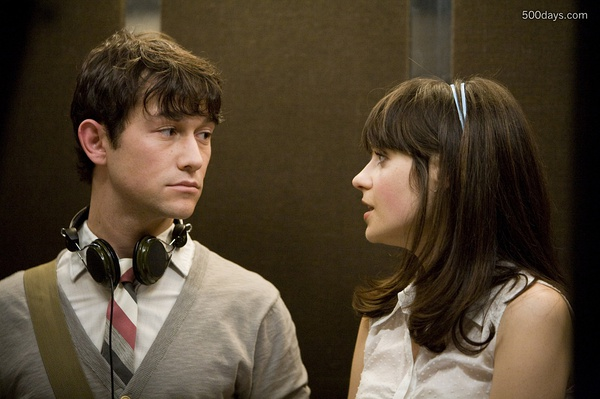
\includegraphics[width=\textwidth]{Zooey2}
        \end{column}
      \end{columns}
    \end{column}
  \end{columns}

\end{frame}
%%%%% ++++++++++++++++++++++++++++++++++++++++++++++++++++++++++++++++++++++++++++++
%% Use the \againframe command to “continue” frames that you previously started
%% somewhere, but where certain details have been suppressed.
%% You can use the \againframe command at a much later point,
%% for example only in the appendix to show additional slides there.
%% In beamer, you can use the \framezoom command to create links to
%% zoomed out parts of a complicated slide.
%% Behind the whole text area (which contains the zoomed area) a big
%% invisible “Back” button is put. Thus clicking anywhere on the text
%% area will jump back to the original (unzoomed) picture.
%% If you do not wish to have the frame title shown on a zoomed slide,
%% you can add an overlay specification to the \frametitle command that
%% simply suppresses the title for the slide. Also, by using the plain option,
%% you can have the zoomed slide fill the whole page.
%%%%% ++++++++++++++++++++++++++++++++++++++++++++++++++++++++++++++++++++++++++++++
\begin{frame}<1>[label=Zooms,fragile, plain]
\frametitle<1>{Zooming Figure}
  \begin{columns}[T]
    \begin{column}{.3\textwidth}
%      \framezoom<1><2>[border](0cm,0cm)(0.5cm,0.5cm)
      \framezoom<1><2>[border](1cm,1cm)(0.5cm,0.5cm)
%      \framezoom<1><4>[border](2cm,2cm)(0.5cm,0.5cm)
%     \pgfimage[height=6cm]{tiger}
      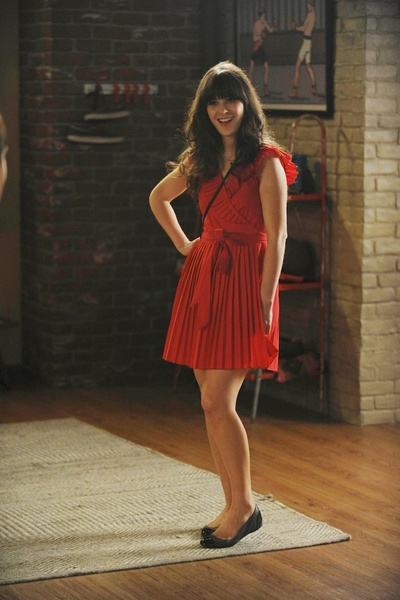
\includegraphics[height=4cm]{Zooey} % is working, too!
    \end{column}

    \begin{column}{.7\textwidth}
      Grammar:
      \begin{itemize}
        \item Figures can be zoomed using
        \item \alert{\path{\framezoom<button overlay><zoomed overlay>[options](x,y)(w,h)}}
        \item options: border.
        \item (x,y): Upper left coordinate point.\\
        They are measures relative to the place where the first normal text of a frame would go.
        Thus, the location $(0pt,0pt)$ is at the beginning of the normal text (which excludes
        the headline and also the frame title).
        \item (w,h): Width and height for zooming.
      \end{itemize}
    \end{column}
  \end{columns}

\end{frame}
%%%%% ++++++++++++++++++++++++++++++++++++++++++++++++++++++++++++++++++++++++++++++
\begin{frame}[label=Wing_A,fragile]
\frametitle{Zooming Figure}

\begin{columns}[T]
\begin{column}{.4\textwidth}

  \begin{figure}
    \centering
    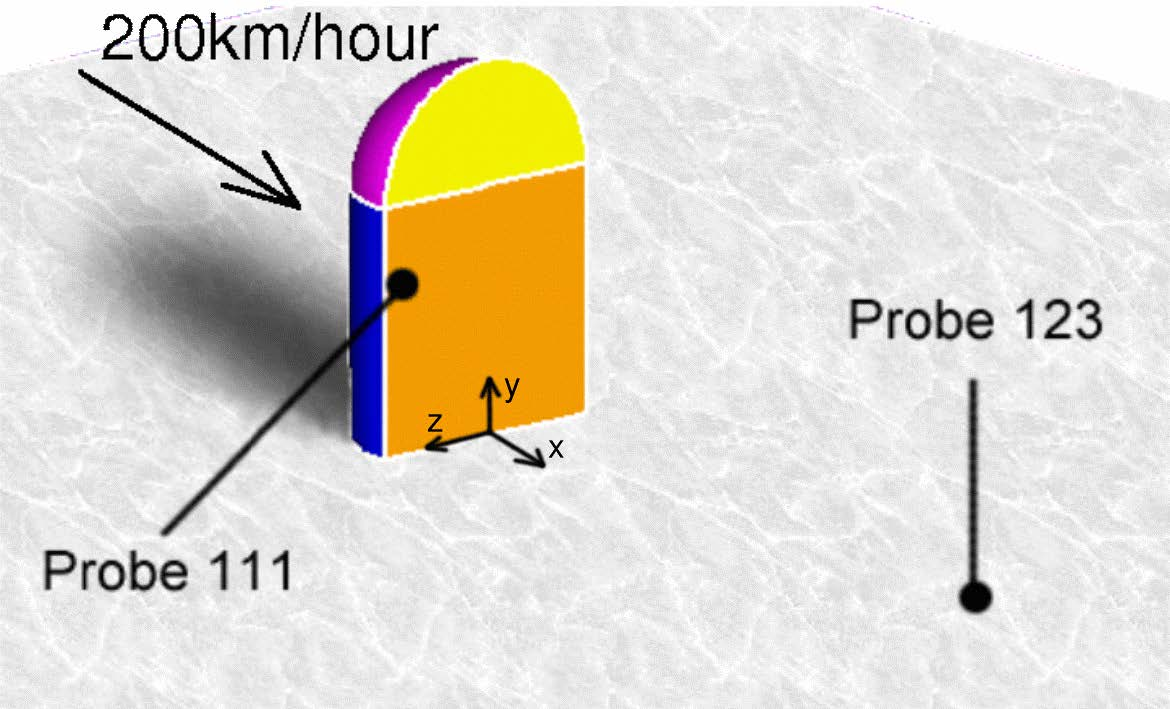
\includegraphics[width=\textwidth]{Wingmirror_Geo}
%   \caption*{{\normalsize Model Geometry}}
  \end{figure}

  \alert{Comments:}

  \begin{itemize}

    \item[*] Agreement is favorable across the spectrum

    \item[*] overestimate the sound pressure at probe 2

  \end{itemize}

\end{column}
\begin{column}{.6\textwidth}

  \begin{figure}
    \raggedleft
    \hyperlink{Wing_B}{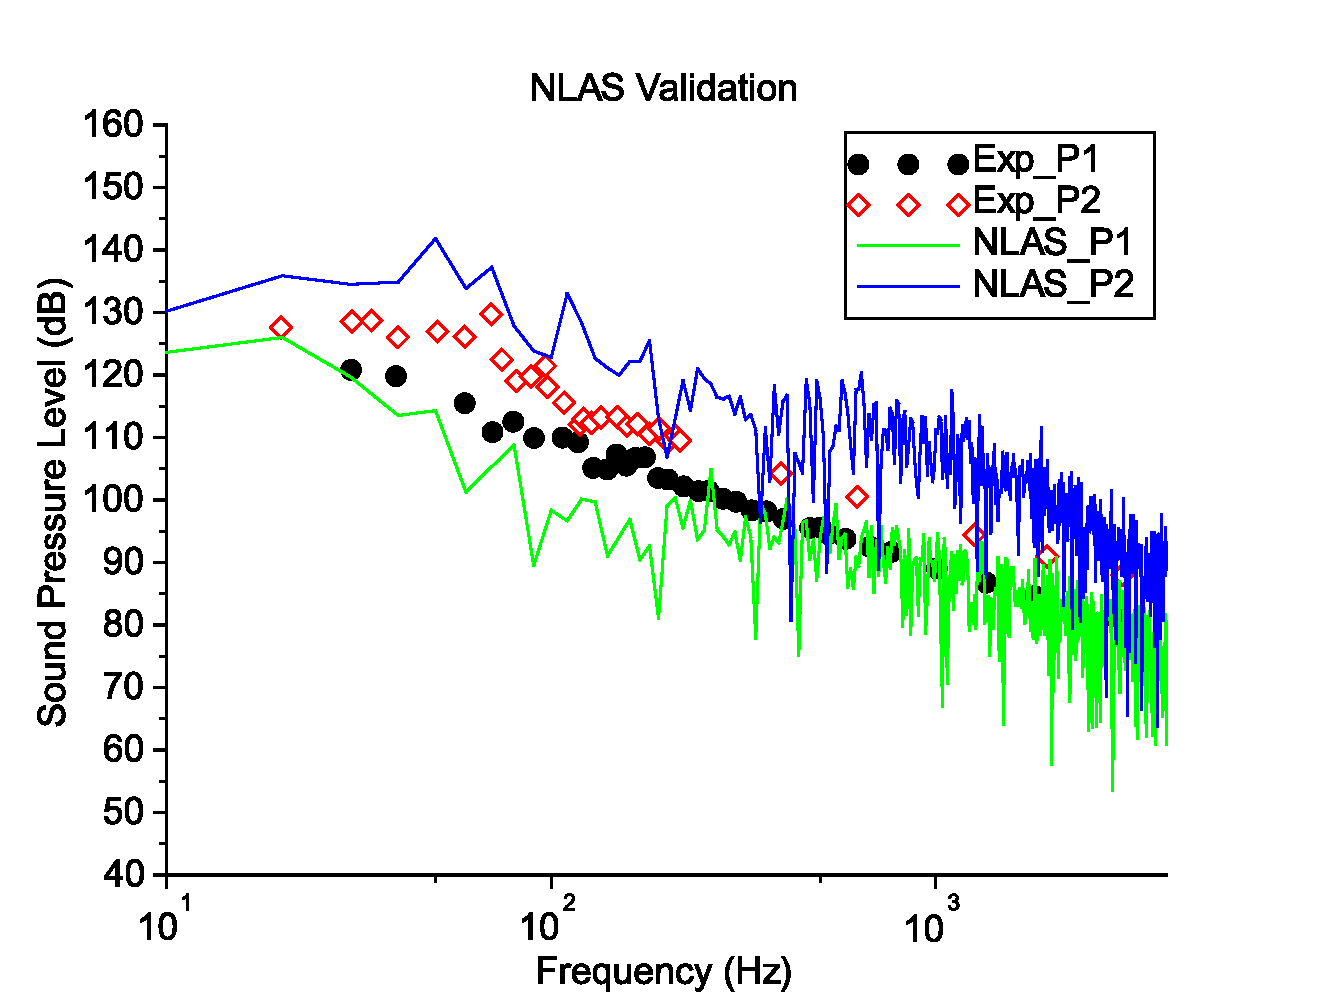
\includegraphics[width=0.9\textwidth]{NLAS_Validation}}
%   \caption*{{\normalsize Model Geometry}}
  \end{figure}

\end{column}
\end{columns}

\note{
  \tiny
  \begin{itemize}
    \item Prediction of flow-induced noise requires a description of all relevant scales of motion
    \item Transmission of the resulting acoustic waves requires a method with minimal dispersion and dissipation
    \item NLAS uses a reconstruction procedure to generate noise sources from the given set of statistics
    \item NLAS allows the propagation of the pressure disturbances to be simulated using a high-resolution pre-conditioned solver.
    \item NLAS is able to predict both broadband and tonal noise
    \item NLAS sub-grid treatment is less diffusive than traditional LES and provides a mechanism to extract acoustic signals from unresolvable eddy foot-prints (sub-grid scale).
    \item LES suits for the noise sources arise from an inherently strong, that numerical and modeled diffusion has little opportunity to overwhelm these disturbances
    \item situations in which the fluid instability is weak and/or arising from scales significantly shorter that the acoustic wavelengths, capturing the relevant noise sources requires greater accuracy and enhanced modeling of unresolved scales.
  \end{itemize}
}
\end{frame}
%%%%% ++++++++++++++++++++++++++++++++++++++++++++++++++++++++++++++++++++++++++++++
\section{Splitting a Frame into Multiple Columns}
%% The main environment for creating columns is called columns.
%% Inside this environment, you can either place several column environments,
%% each of which creates a new column, or use the \column command to
%% create new columns.
%\begin{columns}[options]
%  \begin{column}[pos]{width}
%     ... contents ...
%  \end{column}
%  \begin{column}[pos]{width}
%    ... contents ...
%  \end{column}
%\end{columns}
%% Options:
%% - b will cause the bottom lines of the columns to be vertically aligned.
%% - c will cause the columns to be centered vertically relative to each other.
%%   Default, unless the global option t is used.
%% - onlytextwidth is the same as totalwidth=\textwidth.
%% - t will cause the first lines of the columns to be aligned.
%% - T is similar to the t option, but T aligns the tops of the first lines
%%   while t aligns the so-called baselines of the first lines.
%% - totalwidth=<width> will cause the columns to occupy not the whole
%%   page width, but only <width>, all told.
%% The parameter \linewidth contains the line length inside a list (or derived)
%% environment and it may change in a nested list (while \hsize, \textwidth and
%% \columnwidth don't change). When we have to specify a length depending on current
%% conditions, we have to use the correct parameter. For example, the width of a figure
%% should be specified in terms of \columnwidth in a figure environment and of \textwidth
%% in a figure* environment; however this is done rarely when it's known that
%% the document will be typeset in one column format. The same should be for a tabular* or
%% tabularx environment.
%% Instead, when we need something centered with respect to a line in a list,
%% we should use \linewidth
%% However, in Beamer's column environment:
%% Remark: Within each column, the variable \textwidth is redefined to refer to
%% that column's width. For instance, in the sample shown above, the width of
%% the image is set to 0.7\textwidth which means 0.7 times the width of the column that
%% contains the image.
%% Remark: I find it easier giving widths of columns in terms of fractions of \textwidth.
%% If you wish, however, you may specify absolute widths, such as: \begin{column}{30mm}.
%% For this, you should know that the overall size of a Beamer slide is 128mm x 96mm.
\subsection{Column Environment}
%%%%% ++++++++++++++++++++++++++++++++++++++++++++++++++++++++++++++++++++++++++++++
\begin{frame}[label=ForSkipZoom]
\frametitle{Splitting a slide into Columns}

The line you are reading goes all the way across the slide.
From the left margin to the right margin.  Now we are going
to split the slide into two columns.

\bigskip

\begin{columns}[T]
  \begin{column}{0.5\textwidth}
    Here is the first column.  We put an itemized list in it.
    \begin{itemize}
      \item This is an item
      \item This is another item
      \item Yet another item
    \end{itemize}
  \end{column}

  \begin{column}{0.3\textwidth}
    Here is the second column.  We will put a picture in it.
    \centerline{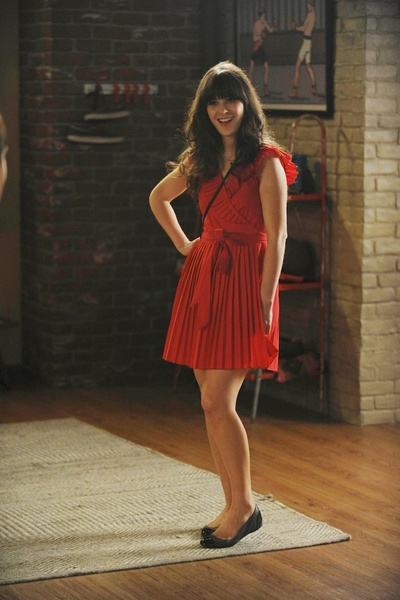
\includegraphics[width=0.7\textwidth]{Zooey}}
  \end{column}
\end{columns}

\bigskip

The line you are reading goes all the way across the slide.

\end{frame}
%%%%% ++++++++++++++++++++++++++++++++++++++++++++++++++++++++++++++++++++++++++++++
\begin{frame}
\frametitle{More More More Columns}

\vfill

\begin{columns}
  \begin{column}{.33\textwidth}
    Left column\\
    blah blah blah blah\\
  \end{column}

  \begin{column}{.33\textwidth}
    Middle column\\
    blah blah blah blah\\
  \end{column}

  \begin{column}{.33\textwidth}
    Right column\\
    blah blah blah blah\\
  \end{column}
\end{columns}

\vfill

\begin{columns}
  \begin{column}{.5\textwidth}
    Bottom Left column\\
    blah blah blah blah\\
  \end{column}

  \begin{column}{.5\textwidth}
    Bottom Right column\\
    blah blah blah blah\\
  \end{column}
\end{columns}

\end{frame}
%%%%% ++++++++++++++++++++++++++++++++++++++++++++++++++++++++++++++++++++++++++++++
\begin{frame}[fragile]
\frametitle{Columns with Graphics \textrm{I}}

\begin{columns}[T]
  \column{5cm}
    Two\\lines.
    \begin{tiny}
      \begin{verbatim}
\begin{columns}[T]
\column{5cm}
  Two\\lines.
\column[c]{5cm}
  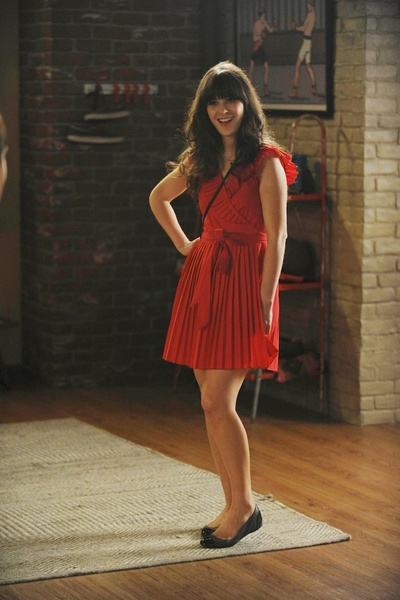
\includegraphics[width=4cm]{Zooey}
\end{columns}
      \end{verbatim}
    \end{tiny}
  \column[c]{5cm}
    \centerline{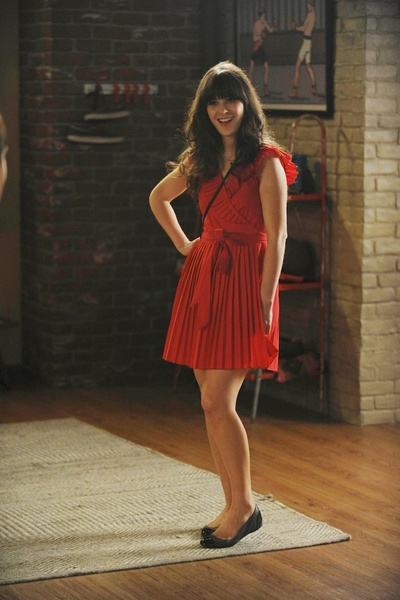
\includegraphics[width=4cm]{Zooey}}
\end{columns}

\end{frame}
%%%%% ++++++++++++++++++++++++++++++++++++++++++++++++++++++++++++++++++++++++++++++
\begin{frame}[fragile]
\frametitle{Columns with Graphics \textrm{II}}

\begin{columns}[c]
  \column{5cm}
    Two\\lines.
    \begin{tiny}
      \begin{verbatim}
\begin{columns}[c]
\column{5cm}
  Two\\lines.
\column[c]{5cm}
  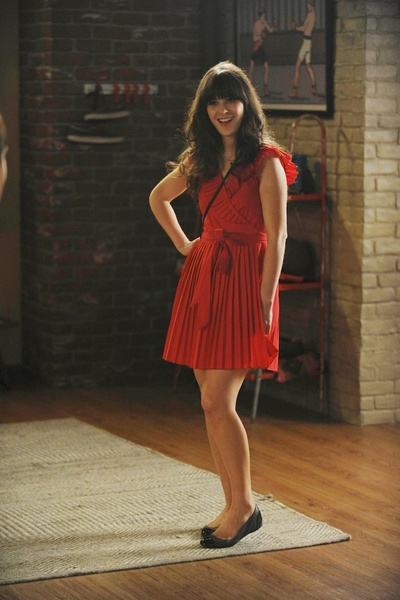
\includegraphics[width=4cm]{Zooey}
\end{columns}
      \end{verbatim}
    \end{tiny}
  \column[c]{5cm}
    \centerline{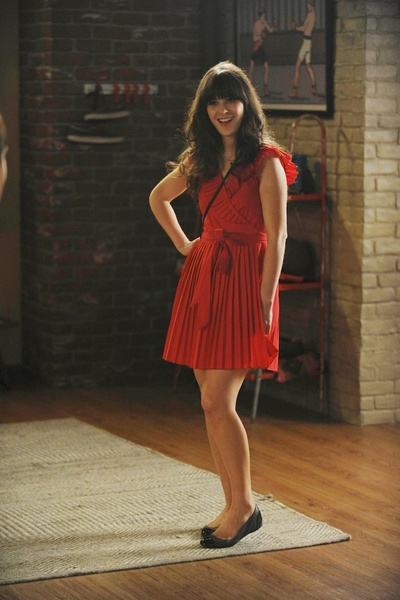
\includegraphics[width=4cm]{Zooey}}
\end{columns}

\end{frame}
%%%%% ++++++++++++++++++++++++++++++++++++++++++++++++++++++++++++++++++++++++++++++
\begin{frame}[plain]
\frametitle{Columns with Graphics \textrm{III}}

\begin{columns}
  \begin{column}[T]{.5\textwidth}
    \centerline{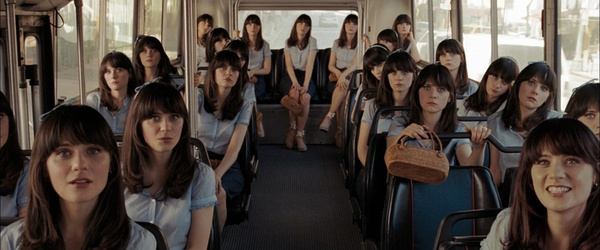
\includegraphics[width=.75\textwidth]{Zooey1}}
  \end{column}

  \begin{column}[T]{.5\textwidth}
    \centerline{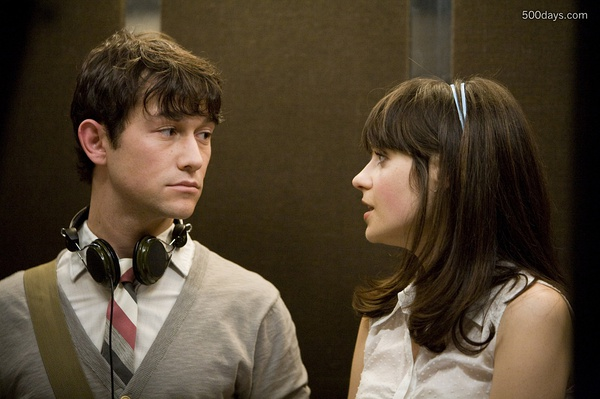
\includegraphics[width=.75\textwidth]{Zooey2}}
  \end{column}
\end{columns}

\vfill

\begin{columns}
  \begin{column}[T]{.5\textwidth}
    \centerline{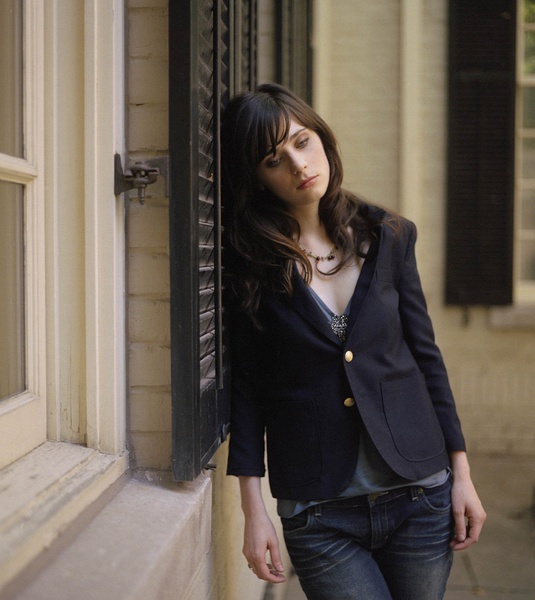
\includegraphics[width=.75\textwidth]{Zooey3}}
  \end{column}

  \begin{column}[T]{.5\textwidth}
    \centerline{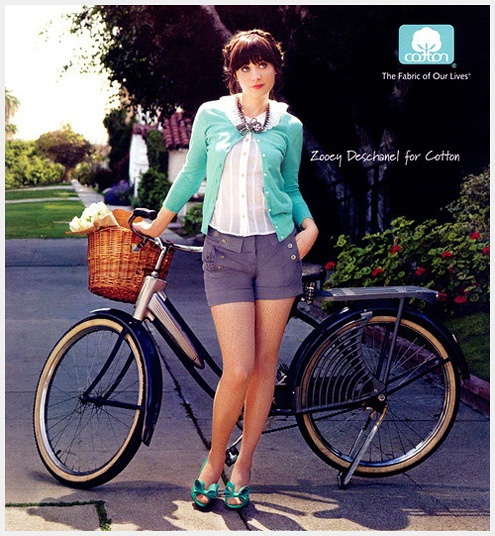
\includegraphics[width=.75\textwidth]{Zooey4}}
  \end{column}
\end{columns}

\end{frame}
%%%%% ++++++++++++++++++++++++++++++++++++++++++++++++++++++++++++++++++++++++++++++
%% You may sometimes wish to have some part of a frame change dynamically from
%% slide to slide. On each slide of the frame, something different should be shown
%% inside this area. You could achieve the effect of dynamically changing text
%% by giving a list of \only commands like this:
%% \only<1>{Initial text.}
%% \only<2>{Replaced by this on second slide.}
%% \only<3>{Replaced again by this on third slide.}
%% The trouble with this approach is that it may lead to slight, but annoying differences
%% in the heights of the lines, which may cause the whole frame to “wobble” from
%% slide to slide. This problem becomes much more severe if the replacement text is
%% several lines long. To solve this problem, you can use two environments: overlayarea and
%% overprint. The first is more flexible, but less user-friendly.
%% \begin{overlayarea}{<area width>}{<area height>}
%%   <environment contents>
%% \end{overlayarea}
%% Everything within the environment will be placed in a rectangular area of
%% the specified size. The area will have the same size on all slides of a frame,
%% regardless of its actual contents.
%% Example:
%% \begin{overlayarea}{\textwidth}{3cm}
%% \only<1>{Some text for the first slide.\\Possibly several lines long.}
%% \only<2>{Replacement on the second slide.}
%% \end{overlayarea}
\begin{frame}
\frametitle{Columns with Graphics \textrm{IV}}

  \begin{columns}
    \begin{column}{.5\textwidth}
      \begin{itemize}
        \item<1-> \emph{Important text}
        \item<2-> Very important process
           \begin{itemize}
             \item<3-> Steps one and two
             \item<5-> Step with no image
           \end{itemize}
      \end{itemize}
    \end{column}
    \begin{column}{.4\textwidth}
        \begin{overlayarea}{\textwidth}{4cm}
%% Here can not use \centerline, adjust the horizonal position of pictures by set
%% different \begin{column}{.4\textwidth}.
%          \includegraphics<2-4>[scale=0.2]{Zooey1}
          \includegraphics<2>[width=\textwidth]{Zooey1}
          \includegraphics<3>[width=\textwidth]{Zooey2}
          \includegraphics<4>[width=\textwidth]{Zooey3}
        \end{overlayarea}
    \end{column}
  \end{columns}

\end{frame}
%%%%% ++++++++++++++++++++++++++++++++++++++++++++++++++++++++++++++++++++++++++++++
\subsection{Minipage Environment}
%% Minipage is an environment providing a paragraph box which is a
%% complete miniversion of a page. It can contain its own footnotes,
%% paragraphs, arrays, tabulars, and other environments. It cannot,
%% however, contain floats or \marginpar commands, but it can appear
%% inside figure or table environments.
%% The syntax is the following:
%% \begin{minipage}[<pos>][<height>][<inner-pos>]{<width>}
%%   <text>
%% \end{minipage}
%% where
%% <pos> controlls the vertical positioning of the box with respect to
%% the text baseline (valid values: c, t, or b).
%% <height> determines the height of the box.
%% <width> determines the width of the box.
%% <inner-pos> determines the position of <text> within the box.
%% The four special length parameters \width, \height, \depth, and
%% \totalheight (= \height + \depth) specify the natural size of <text>.
%%%%% ++++++++++++++++++++++++++++++++++++++++++++++++++++++++++++++++++++++++++++++
\begin{frame}
\frametitle{Test Minipage \textrm{I}}

  \begin{columns}
    \column{.5\textwidth}
      \centerline{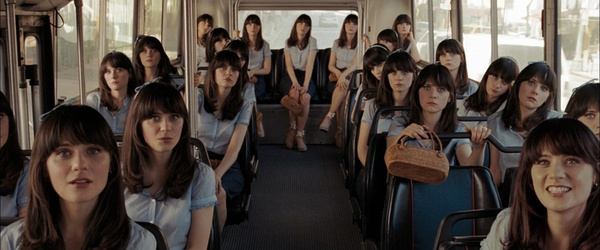
\includegraphics[scale = 0.2]{Zooey1}}
    \column{.5\textwidth}
      \begin{minipage}[c][.6\textheight][c]{\linewidth}
        \begin{itemize}
          \item Item 1
          \item Item 2
        \end{itemize}
      \end{minipage}
  \end{columns}

\end{frame}
%%%%% ++++++++++++++++++++++++++++++++++++++++++++++++++++++++++++++++++++++++++++++
\begin{frame}
\frametitle{Test Minipage \textrm{II}}

  \begin{columns}
    \column{.5\textwidth}
      \centerline{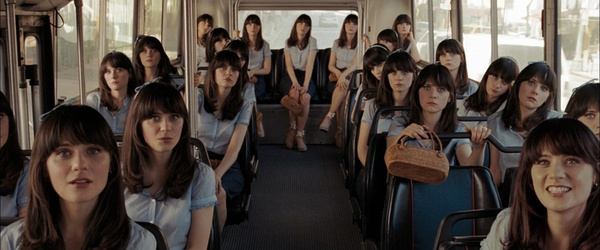
\includegraphics[scale = 0.2]{Zooey1}}
    \column{.5\textwidth}
      \begin{minipage}[c][.6\textheight][c]{\linewidth}
        \begin{itemize}
          \item<1-> Another item 1
          \item<2-> Another item 2
          \item<3-> This list is longer
          \item<4-> Than the previous one.
        \end{itemize}
      \end{minipage}
  \end{columns}

\end{frame}
%%%%% ++++++++++++++++++++++++++++++++++++++++++++++++++++++++++++++++++++++++++++++
\section{Tables}
%% The 'l c r' on the first line indicates that the first, second,
%% and third columns should be left-justified, centered,
%% and right-justified, respectively.
%% double backslashes (\\) tell LaTeX where the end of a row is
%% the ampersand (&) marks the dividing line between columns.
%%%%% ++++++++++++++++++++++++++++++++++++++++++++++++++++++++++++++++++++++++++++++
\begin{frame}[fragile]
\frametitle{A Simple One}

  \begin{columns}
    \begin{column}{.5\textwidth}
      \begin{scriptsize}
\begin{verbatim}
\begin{center}
  \begin{tabular}{ l | c || r | }
    \hline
    1 & 2 & 3 \\
    \hline
    4 & 5 & 6 \\
    7 & 8 & 9 \\
    \hline
  \end{tabular}
\end{center}
\end{verbatim}
      \end{scriptsize}
    \end{column}

    \begin{column}{.4\textwidth}
      \begin{center}
        \begin{tabular}{ l | c || r | }
          \hline
          1 & 2 & 3 \\
          \hline
          4 & 5 & 6 \\
          7 & 8 & 9 \\
         \hline
        \end{tabular}
      \end{center}
    \end{column}
  \end{columns}

\end{frame}
%%%%% ++++++++++++++++++++++++++++++++++++++++++++++++++++++++++++++++++++++++++++++
\begin{frame}[fragile]
\frametitle{More Complicated}

  \begin{columns}
    \begin{column}{.5\textwidth}
      \begin{scriptsize}
\begin{verbatim}
\begin{center}
  \begin{tabular}{|r|l|}
    \hline
    7C0 & hexadecimal \\
    3700 & octal \\ \cline{2-2}
    11111000000 & binary \\
    \hline \hline
    1984 & decimal \\
    \hline
  \end{tabular}
\end{center}
\end{verbatim}
      \end{scriptsize}
    \end{column}

    \begin{column}{.5\textwidth}
      \begin{center}
        \begin{tabular}{|r|l|}
          \hline
          7C0 & hexadecimal \\
          3700 & octal \\ \cline{2-2}
          11111000000 & binary \\
          \hline \hline
          1984 & decimal \\
          \hline
        \end{tabular}
      \end{center}
    \end{column}
  \end{columns}

\end{frame}
%%%%% ++++++++++++++++++++++++++++++++++++++++++++++++++++++++++++++++++++++++++++++
\begin{frame}[fragile]
\frametitle{Even More Complicated}

  \begin{columns}
    \begin{column}{\textwidth}
      \begin{scriptsize}
\begin{verbatim}
\begin{center}
  \begin{tabular}{ l | c || r | }
    \hline
    \onslide<2-6,8>{1} & \onslide<3-6>{2} & \onslide<4-6,9>{hello} \\
    \hline
    \onslide<5-6>{4} & \onslide<5-6,8,9>{5} & \onslide<5-6>{6} \\
    \onslide<6,9>{7} & \onslide<6>{8} & \onslide<6,8>{9} \\
    \hline
  \end{tabular}
\end{center}
\end{verbatim}
      \end{scriptsize}
    \end{column}
  \end{columns}

  \begin{columns}
    \begin{column}{.6\textwidth}

    \end{column}

    \begin{column}{.4\textwidth}
      \begin{center}
        \begin{tabular}{ l | c || r | }
          \hline
          \onslide<2-6,8>{1} & \onslide<3-6>{2} & \onslide<4-6,9>{hello} \\
          \hline
          \onslide<5-6>{4} & \onslide<5-6,8,9>{5} & \onslide<5-6>{6} \\
          \onslide<6,9>{7} & \onslide<6>{8} & \onslide<6,8>{9} \\
          \hline
        \end{tabular}
      \end{center}
    \end{column}
  \end{columns}

\end{frame}
%%%%% ++++++++++++++++++++++++++++++++++++++++++++++++++++++++++++++++++++++++++++++
\section{Creating Overlays}
%% The General Concept of Overlay Specifications
%% The idea is to add overlay specifications to certain commands.
%% These specifications are always given in pointed brackets and
%% follow the command “as soon as possible,” though in certain cases
%% beamer also allows overlay specification to be given a little later.
%% In the simplest case, the specification contains just a number.
%% A command with an overlay specification following it will
%% only have “effect” on the slide(s) mentioned in the specification.
%% Consider the following example.
%% \begin{frame}
%% \textbf{This line is bold on all three slides.}
%% \textbf<2>{This line is bold only on the second slide.}
%% \textbf<3>{This line is bold only on the third slide.}
%% \end{frame}
%% For the command \textbf, the overlay specification causes the text
%% to be set in boldface only on the specified slides.
%% On all other slides, the text is set in a normal font.
%% For a second example, consider the following frame:
%% \begin{frame}
%% \only<1>{This line is inserted only on slide 1.}
%% \only<2>{This line is inserted only on slide 2.}
%% \end{frame}
%% The command \only, which is introduced by beamer, normally simply
%% inserts its parameter into the current frame.
%% However, if an overlay specification is present, it “throws away”
%% its parameter on slides that are not mentioned.
%% The syntax of (basic) overlay specifications is the following:
%% They are comma-separated lists of slides and ranges.
%% Ranges are specified like this: 2-5, which means slide two through to five.
%% The start or the end of a range can be omitted.
%% For example, 3- means “slides three, four, five, and so on” and
%% -5 means the same as 1-5. A complicated example is -3,6-8,10,12-15,
%% which selects the slides 1, 2, 3, 6, 7, 8, 10, 12, 13, 14, and 15.
\subsection{Stepwise Viewing}
%%%%% ++++++++++++++++++++++++++++++++++++++++++++++++++++++++++++++++++++++++++++++
%% The pause command offers an easy, but not very flexible way of creating frames that
%% are uncovered piecewise. If you say \pause somewhere in a frame, only the text on the
%% frame up to the \pause command is shown on the first slide. On the second slide,
%% everything is shown up to the second \pause, and so forth.

\begin{frame}[fragile]
\frametitle{Pause for Stepwise Viewing}

  \begin{columns}
    \begin{column}[T]{2in} % begin left column
      \begin{tiny}
        \begin{verbatim}
\begin{itemize}
\item
  Shown from first slide on.
\pause
\item
  Shown from second slide on.
  \begin{itemize}
  \item
    Shown from second slide on.
  \pause
  \item
    Shown from third slide on.
  \end{itemize}
\item
  Shown from third slide on.
\pause
\item
  Shown from fourth slide on.
\end{itemize}
Shown from fourth slide on.
\begin{itemize}
\onslide
\item
  Shown from first slide on.
\pause
\item
  Shown from fifth slide on.
\end{itemize}
        \end{verbatim}
      \end{tiny}
    \end{column} % end left column

    \begin{column}[T]{2.2in} % begin right column
      \begin{itemize}
        \item
          Shown from first slide on.
        \pause
        \item
          Shown from second slide on.
          \begin{itemize}
            \item
              Shown from second slide on.
            \pause
            \item
              Shown from third slide on.
          \end{itemize}
        \item
          Shown from third slide on.
        \pause
        \item
          Shown from fourth slide on.
      \end{itemize}

      Shown from fourth slide on.

      \begin{itemize}
        \onslide
        \item
          Shown from first slide on.
        \pause
        \item
          Shown from fifth slide on.
      \end{itemize}
        \pause
        Note that pause does not know \textcolor{Violet}{overlay counters}.
    \end{column} % end right column
  \end{columns}
\end{frame}
%%%%% ++++++++++++++++++++++++++++++++++++++++++++++++++++++++++++++++++++++++++++++
\begin{frame}[fragile]
\frametitle{Pause: Table Example}%

  \begin{itemize}
    \item Row increment in a table:\pause \\
      \medskip
      \rowcolors[]{1}{blue!20}{blue!10}
      \begin{tabular}{l!{\vrule}cccc}
        Class & A & B & C & D \\\hline
        X & 1 & 2 & 3 & 4 \pause \\
        Y & 3 & 4 & 5 & 6 \pause \\
        Z & 5 & 6 & 7 & 8
      \end{tabular}
    \vfill
    \item Source code:
      \begin{footnotesize}
        \begin{verbatim}
\rowcolors[]{1}{blue!20}{blue!10}
\begin{tabular}{l!{\vrule}cccc}
  Class & A & B & C & D \\\hline
  X & 1 & 2 & 3 & 4 \pause \\
  Y & 3 & 4 & 5 & 6 \pause \\
  Z & 5 & 6 & 7 & 8
\end{tabular}
        \end{verbatim}
      \end{footnotesize}
  \end{itemize}

\end{frame}
%%%%% ++++++++++++++++++++++++++++++++++++++++++++++++++++++++++++++++++++++++++++++
\begin{frame}[fragile]
\frametitle{Onslide for Stepwise Viewing}

  \begin{itemize}
    \item \textcolor{Violet}{\path{\onslide<n-> stuff}} shows stuff on the given slides.%\pause
    \item Example: Column increment in a table:\\%\pause \\
      \rowcolors[]{1}{blue!20}{blue!10}
      \begin{tabular}{l!{\vrule}c<{\onslide<2->}c<{\onslide<3->} %
        c<{\onslide<4->}c<{\onslide}c}
        Class & A & B & C & D \\
        X & 1 & 2 & 3 & 4 \\
        Y & 3 & 4 & 5 & 6 \\
        Z & 5 & 6 & 7 & 8
      \end{tabular}
    \item Source code:\\
      \begin{footnotesize}
        \begin{verbatim}
\rowcolors[]{1}{blue!20}{blue!10}
\begin{tabular}{l!{\vrule}c<{\onslide<2->}c<{\onslide<3->}%
    c<{\onslide<4->}c<{\onslide}c}
    Class & A & B & C & D \\
    X & 1 & 2 & 3 & 4 \\
    Y & 3 & 4 & 5 & 6 \\
    Z & 5 & 6 & 7 & 8
\end{tabular}
        \end{verbatim}
      \end{footnotesize}
  \end{itemize}

\end{frame}
%%%%% ++++++++++++++++++++++++++++++++++++++++++++++++++++++++++++++++++++++++++++++
\begin{frame}[fragile]
\frametitle{Item for Step Viewing \rm{I}}%

  {\color{Violet}\path{item<n->}} for incremental overlays with overlay counters.

\rule{\linewidth}{0.5mm}

  \begin{tabular}{p{.5\textwidth} p{.4\textwidth}}
    \begin{verbatim}
\begin{itemize}
  \item<2-> Every thing
  \item<3-> that has
  \item<4-> beginning
  \item<5-> and end.
\end{itemize}
    \end{verbatim}
    &
    \begin{itemize}
      \item<2-> Every thing
      \item<3-> that has
      \item<4-> beginning
      \item<5-> has end.
    \end{itemize}
  \end{tabular}

\rule{\linewidth}{0.5mm}

  \onslide<6->{\path{\item<n1-n2>} for fine control of overlays.}

\end{frame}
%%%%% ++++++++++++++++++++++++++++++++++++++++++++++++++++++++++++++++++++++++++++++
\begin{frame}[fragile]
\frametitle{Item for Step Viewing \rm{II}}%

  {\color{Violet}\path{<+->}} for incremental overlays automaticlly.

\rule{\linewidth}{0.5mm}

  \begin{tabular}{p{.5\textwidth} p{.4\textwidth}}
    \begin{verbatim}
\begin{itemize}[<+->]
  \item Every thing
  \item that has
  \item beginning
  \item and end.
\end{itemize}
    \end{verbatim}
    &
    \begin{itemize}[<+->]
      \item Every thing
      \item that has
      \item beginning
      \item has end.
    \end{itemize}
  \end{tabular}

\rule{\linewidth}{0.5mm}

\end{frame}
%%%%% ++++++++++++++++++++++++++++++++++++++++++++++++++++++++++++++++++++++++++++++
\subsection{Replace}
%%%%% ++++++++++++++++++++++++++++++++++++++++++++++++++++++++++++++++++++++++++++++
\begin{frame}[fragile]
\frametitle{Replace}%

  \begin{itemize}
    \item Successive \alert{\path{\only<n>{...}}}.\\
      {\scriptsize \path{(Ex)\only<1>{Only1}\only<2>{Only2}\only<3>{Only3}} $\Rightarrow$  \only<1>{Only1}\only<2>{Only2}\only<3>{Only3}}
    \item \alert{\path{\uncover<n>{...}}} shows at given n.\\
      {\scriptsize \path{(Ex)\uncover<5>{I am 5}} $\Rightarrow$ \uncover<5>{I am 5}}
    \item \alert{\path{\invisible<n>{...}}} hides at given n.\\
      {\scriptsize \path{(Ex)\invisible<8>{Invisible at 8}} $\Rightarrow$ \invisible<8>{Invisible at 8}}
    \item \alert{\path{\alt<n>{at n}{not at n}}} for two alternatives.\\
      {\scriptsize \path{(Ex)\alt<11>{I am 11}{I am not 11}} $\Rightarrow$ \alt<11>{I am 11}{I am not 11}}
    \item \alert{\path{\temporal<n>{before}{at n}{after}}} for three alternatives.\\
      {\scriptsize \path{(Ex)\temporal<14>{I am 13}{I am 14}{I am 15}} $\Rightarrow$ \temporal<14>{I am 13}{I am 14}{I am 15}}
  \end{itemize}

  \bigskip

  \begin{center}
    Slide\only<1>{1}\only<2>{2}\only<3>{3}\only<4>{4}\only<5>{5}\only<6>{6}\only<7>{7}\only<8>{8}%
    \only<9>{9}\only<10>{10}\only<11>{11}\only<12>{12}\only<13>{13}\only<14>{14}\only<15>{15}
  \end{center}

\end{frame}
%%%%% ++++++++++++++++++++++++++++++++++++++++++++++++++++++++++++++++++++++++++++++
\begin{frame}[fragile]
\frametitle{More Replaces}%

  In case if subtle differences in the heights of replacements, it may lead to slight, but annoying differences in the heights of the lines, which may cause the whole frame to "wobble" from slide to slide. To solve this problem, {\color{red} overlayarea} and {\color{red}overprint} environment can be used.

  \bigskip

  Example:

  \bigskip

  \begin{overlayarea}{\textwidth}{1.5cm}
    \only<1>{Some text for the first slide.\\Possibly several lines long.}
    \only<2>{Replacement on the second slide.}
  \end{overlayarea}

  \medskip

  \begin{footnotesize}
    \begin{verbatim}
\begin{overlayarea}{\textwidth}{3cm}
  \only<1>{Some text for the first slide.\\
           Possibly several lines long.}
  \only<2>{Replacement on the second slide.}
\end{overlayarea}
    \end{verbatim}
  \end{footnotesize}

\end{frame}
%%%%% ++++++++++++++++++++++++++++++++++++++++++++++++++++++++++++++++++++++++++++++
\begin{frame}[fragile]
\frametitle{Environments with Overlay Specifications}%

\begin{columns}
  \begin{column}{.3\textwidth}
    \begin{theorem}<1->
      Exists infinite set.
    \end{theorem}

    \begin{proof}<3->
      Axiom of infinity.
    \end{proof}

    \begin{example}<2->
      Natural numbers.
    \end{example}
  \end{column}
  \begin{column}{.6\textwidth}
    \begin{scriptsize}
      \begin{verbatim}
\begin{theorem}<1->
  Exists infinite set.
\end{theorem}
\begin{proof}<3->
  Axiom of infinity.
\end{proof}
\begin{example}<2->
  Natural numbers.
\end{example}
      \end{verbatim}
    \end{scriptsize}
    \begin{alertblock}<4->{Note}
      \Tiny
      Various overlay counters: 'n', 'n-', '-n', 'n1-n2', '+-'.
      \begin{verbatim}
\textbf, \textit, \textsl,
\textrm, \textsf, and
\color also understand overlays.
      \end{verbatim}
    \end{alertblock}
  \end{column}
\end{columns}

\end{frame}
%%%%% ++++++++++++++++++++++++++++++++++++++++++++++++++++++++++++++++++++++++++++++
\subsection{Highlighting}
%%%%% ++++++++++++++++++++++++++++++++++++++++++++++++++++++++++++++++++++++++++++++
\begin{frame}[fragile]
\frametitle{Simple Highlighting}%

  {\color{Violet}\path{\item<+-| alert@+>}} for automatic highlighting.

\rule{\linewidth}{0.5mm}

  \begin{columns}
    \footnotesize
    \begin{column}{.5\textwidth}
      \begin{verbatim}
\begin{itemize}
  \item <+-| alert@+> Every thing
  \item <+-| alert@+> that has
  \item <+-| alert@+> beginning
  \item <+-| alert@+> has end.
\end{itemize}
      \end{verbatim}
    \end{column}

    \begin{column}{.3\textwidth}
      \begin{itemize}
        \item <+-| alert@+> Every thing
        \item <+-| alert@+> that has
        \item <+-| alert@+> beginning
        \item <+-| alert@+> has end.
      \end{itemize}
    \end{column}
  \end{columns}

\rule{\linewidth}{0.5mm}

  \begin{itemize}
    \item You can also use {\color{Violet}\path{\begin{itemize}[<+-|alert@+>]}} instead of individual '{\color{Violet}\path{\item<+-|alert@+>}}'.
    \item You can use {\color{Violet}structure} instead of {\color{Violet}alert}.
  \end{itemize}

\end{frame}
%%%%% ++++++++++++++++++++++++++++++++++++++++++++++++++++++++++++++++++++++++++++++
\begin{frame}[fragile]
\frametitle{Alert for Highlighting}%

  {\color{Violet}\path{\item<n->\alert<m>{stuff}}} is better than the previous automatic one.

\rule{\linewidth}{0.5mm}

  \begin{columns}
    \footnotesize
    \begin{column}{.5\textwidth}
      \begin{verbatim}
\begin{itemize}
  \item<1->\alert<2> {Every thing}
  \item<1->\alert<3> {that has}
  \item<1->\alert<4> {beginning}
  \item<1->\alert<5> {has end.}
\end{itemize}
      \end{verbatim}
    \end{column}

    \begin{column}{.3\textwidth}
      \begin{itemize}
        \item<1->\alert<2> {Every thing}
        \item<1->\alert<3> {that has}
        \item<1->\alert<4> {beginning}
        \item<1->\alert<5> {has end.}
      \end{itemize}
    \end{column}
  \end{columns}

\rule{\linewidth}{0.5mm}

  Note that {\color{Violet}\path{\item<1->\alert<2>}} is same to {\color{Violet}\path{\item<1-| alert@2>}}.

\end{frame}
%%%%% ++++++++++++++++++++++++++++++++++++++++++++++++++++++++++++++++++++++++++++++
\begin{frame}[fragile]
\frametitle{Temporal for Highlighting}%

  \begin{itemize}
    \item {\color{Violet}\path{\temporal<n>{before}{on}{after}}} for highlighting
    \item Ready?\\
      \begin{itemize}
        \hilite<2> \item Everything
        \hilite<3> \item that has
        \hilite<4> \item beginning
        \hilite<5> \item has end.
      \end{itemize}
    \item Source code:\\
      \begin{scriptsize}
        \begin{verbatim}
\def\hilite<#1>{%
\temporal<#1>{\color{gray}}{\color{blue}}%
{\color{blue!25}}}
...
\begin{itemize}
  \hilite<3> \item Everything
  \hilite<4> \item that has
  \hilite<5> \item beginning
  \hilite<6> \item has end.
\end{itemize}
        \end{verbatim}
      \end{scriptsize}
  \end{itemize}

\end{frame}
%%%%% ++++++++++++++++++++++++++++++++++++++++++++++++++++++++++++++++++++++++++++++
\section{Hyperlinks and Buttons}
%%%%% ++++++++++++++++++++++++++++++++++++++++++++++++++++++++++++++++++++++++++++++
\begin{frame}[fragile]
\frametitle{Hyperlinks and Buttons}%

  \begin{itemize}
    \small
    \item Beamer provides additional options for hyperlinks and buttons.
    \item {\color{Violet}\path{\hyperlink{targetname}{\beamergotobutton{text}}}} to create link.
    \item {\color{Violet}\path{\hypertarget{targetname}{text}}} to create target.
    \item To make a button "clickable" you must place it in a command like \path{\hyperlink}.
    \item Some useful buttons are \path{\beamerbutton}, \path{\beamergotobutton}, \path{\beamerreturnbutton} and \path{\beamerskipbutton}.
    \item To go to the title page, click \hfill \hyperlinkpresentationstart{\beamerbutton{\color{red}Title Page}}
    \item To go to the end of presentation, click \hfill \hyperlinkpresentationend{\beamerbutton{\color{red}End Page}}
    \item To go to the appendix, click \hfill \hyperlinkappendixstart{\beamerbutton{\color{red}Appendix}}
  \end{itemize}

\end{frame}
%%%%% ++++++++++++++++++++++++++++++++++++++++++++++++++++++++++++++++++++++++++++++
\begin{frame}[fragile]
\frametitle{Beamer Skip Button}%

  The symbol drawn for this button is usually a double right arrow. Use this button if pressing it will skip over a well-defined part of your talk.

  \begin{theorem}
    I got a theorem.
  \end{theorem}

%% \begin{overprint}[<area width>]
%%    <environment contents>
%% \end{overprint}
%% The <area width> defaults to the text width. Inside the environment,
%% use \onslide commands to specify different things that should be shown
%% for this environment on different slides. Everything within the environment
%% will be placed in a rectangular area of the specified width. The height and
%% depth of the area are chosen large enough to accommodate the largest
%% contents of the area.

  \begin{overprint}
    \onslide<1>
    \hfill\hyperlinkframestartnext{\beamerskipbutton{Skip proof}}
    \onslide<2>
    \begin{proof}
      I am trying...
    \end{proof}
  \end{overprint}

\end{frame}
%%%%% ++++++++++++++++++++++++++++++++++++++++++++++++++++++++++++++++++++++++++++++
\begin{frame}<1>[fragile,label=mytheorem]
\frametitle{Beamer Goto and Return Button}%

  \begin{theorem}
    I got a theorem...
  \end{theorem}
  \begin{overprint}
    \onslide<1>
      \hfill\hyperlink{mytheorem<2>}{\beamergotobutton{Go to proof details}}
    \onslide<2>
    \begin{proof}
      This is the proof details attached in Appendix.
    \end{proof}
    \hfill\hyperlink{mytheorem<1>}{\beamerreturnbutton{Return}}
  \end{overprint}
%% need to use \againframe<2>{mytheorem} in Appendix part. i.e., after \appendix.
\end{frame}
%%%%% ------------------------------------------------------------------------------
\section{Animations}
%%%%% ++++++++++++++++++++++++++++++++++++++++++++++++++++++++++++++++++++++++++++++
\begin{frame}[fragile]
\frametitle{Animations Created by Showing Slides in Rapid Succession}%

  \begin{itemize}
    \scriptsize
    \item To facilitate the creation of animations using this feature, the following commands can be used: {\color{Violet}\path{\animate}} and {\color{Violet}\path{\animatevalue}}.
    \item \path{\animate<overlay specification>} \\ The slides specified by \emph{overlay specification} will be shown as quickly as possible.
    \item \path{\animatevalue<start slide-end slide>{name}{start value}{end value}}\\The \emph{name} must be the name of a \emph{counter} or a \emph{dimension}. It will be varied between two values. For the slides in the specified range, the counter or dimension is set to an interpolated value that depends on the current slide number. On slides before the \emph{start slide} the counter or dimension is set to \emph{start value}, on the slides after the \emph{end slide} it is set to \emph{end value}.
    \item Use with caution as animation needs lots of slides.
    \item For Acrobat Adobe Reader, this works only in full-screen mode.
  \end{itemize}

\end{frame}
%%%%% ++++++++++++++++++++++++++++++++++++++++++++++++++++++++++++++++++++++++++++++
\begin{frame}
\frametitle{A Five Slide Animation with \path{\animate<n1-n2>}}

  \animate<2-4>

  The first slide is shown normally. When the second slide is shown (presumably after pressing a forward key), the second, third, and fourth slides "flash by" At the end, the content of the fifth slide is shown.

  \bigskip

  \begin{itemize}[<+->]
    \item Everything
    \item that has
    \item beginning
    \item has end.
    \item That's right!
  \end{itemize}

\end{frame}
%
%%
%%% >>> Backmatter
%%
%% Matters of Bibliography, Glossary, Index.
%%%%% ++++++++++++++++++++++++++++++++++++++++++++++++++++++++++++++++++++++++
\section*{}% Backmatter
%%%%% ++++++++++++++++++++++++++++++++++++++++++++++++++++++++++++++++++++++++
%%
%% >>> Bibliography
%%
%%%%%% ++++++++++++++++++++++++++++++++++++++++++++++++++++++++++++++++++++++++
%\begin{frame}[allowframebreaks]
%    \frametitle{}
%    \tiny
%    \printbibliography
%\end{frame}
%%%%% ++++++++++++++++++++++++++++++++++++++++++++++++++++++++++++++++++++++++
%%
%% >>> The End Page
%%
\subsection*{}% the end page.
%%%%% ++++++++++++++++++++++++++++++++++++++++++++++++++++++++++++++++++++++++
{
    \logo{\includegraphics[height=0.10\textwidth]{logo}}
    \begin{frame}
        \begin{center}
            {\Huge \textcolor{black}{Thanks for your attention!}}
        \end{center}
    \end{frame}
}
%%%%% ++++++++++++++++++++++++++++++++++++++++++++++++++++++++++++++++++++++++
%%
%% >>> Appendix
%%
\appendix% begin appendix
\newcounter{finalframe} % define a new counter
\setcounter{finalframe}{\value{framenumber}} % save regular slides counter
\section{\appendixname}% the end page.
\frame{\tableofcontents}% outline for appendix
%%%%% ++++++++++++++++++++++++++++++++++++++++++++++++++++++++++++++++++++++++
\subsection{Additional Material}
%%%%% ++++++++++++++++++++++++++++++++++++++++++++++++++++++++++++++++++++++++
\begin{frame}[fragile]
    \frametitle{Further Reading}%

    \begin{itemize}
        \item The Wikibooks
        \item Beamer's User Guide
    \end{itemize}

\end{frame}
%%%%% ++++++++++++++++++++++++++++++++++++++++++++++++++++++++++++++++++++++++
%% proof details
\againframe<2>{mytheorem}
%% zoom figure
\againframe<2->[plain]{Zooms}
%%%%% ++++++++++++++++++++++++++++++++++++++++++++++++++++++++++++++++++++++++
\begin{frame}[fragile,label=Wing_B,plain]
    %\frametitle{Zooming Figure}
    \begin{figure}
        \centering
        \hyperlink{Wing_A}{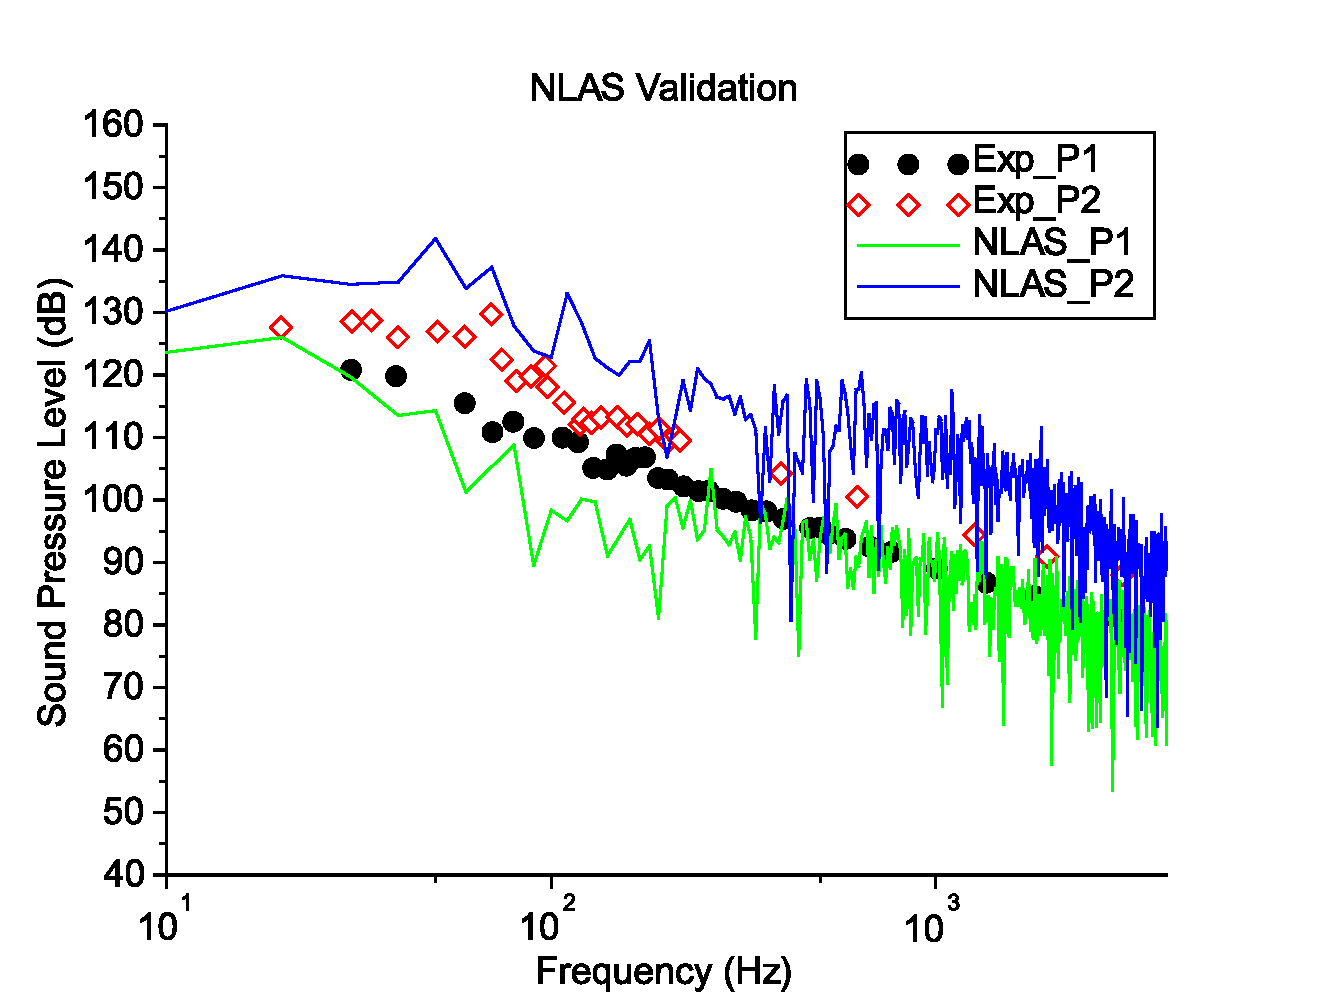
\includegraphics[width=\textwidth]{NLAS_Validation}}
        %   \caption*{{\normalsize Model Geometry}}
    \end{figure}
\end{frame}
%%%%% ++++++++++++++++++++++++++++++++++++++++++++++++++++++++++++++++++++++++
\setcounter{framenumber}{\value{finalframe}} % rectify the slides counter
%%%%% ++++++++++++++++++++++++++++++++++++++++++++++++++++++++++++++++++++++++

%%
\end{document}
%%%%% --------------------------------------------------------------------------------
